\textbf{De organisatie is ingericht om de betrouwbaarheidsrisico's niet uit te laten komen. Bij de analyse van de betrouwbaarheidsrisico's is nodig om duidelijk te krijgen wat de gevolgen zouden zijn wanneer de risico's uitkomen, maar ook de kans waarop deze risico's kunnen gebeuren. De risico's zijn verschillend per proces, afdeling, doel, soort organisatie, en typologie. Hoewel een aantal betrouwbaarheidsrisico's inherent zijn aan de werkzaamheden van de onderneming, kunnen er ook nieuwe risico's ter sprake komen door bijvoorbeeld een toename van het aantal medewerkers, een nieuwe organisatiestructuur, acquisitie van andere ondernemingen, een buitengewone groei, nieuwe producten en/of afdelingen.}

\subsection{Het COSO-raamwerk}
Allereerst speelt het COSO raamwerk van principes voor interne controle. In tabel \ref{tab:risicoprincipes} is het vervolg van het eerder besproken raamwerk te vinden. Een viertal principes kunnen hiermee de verschillende soorten organisaties typeren. 

\begin{table}[h]
    \centering
    \caption{Excerpt van de principes voor interne controle volgens COSO}
    \begin{tabular}{l l}
        \toprule
        \textbf{Element} & \textbf{Principe} \\
        \midrule
        Risico analyse & 6. Specificeert relevante doelstellingen \\
         & 7. Identificeert relevante doelstellingen \\
         & 8. Fraudebewustzijn \\
         & 9. Identificeert en analyseert belangrijke wijzigingen \\
        \bottomrule
    \end{tabular}
    \label{tab:risicoprincipes}
\end{table}

Er is hier gekozen voor principe 9. Ten behoeve van de primaire processen (met name: inkoop, voorraad, en verkoop) geeft de leiding aan snel te kunnen schakelen als het gaat over nieuwe kansen. Er wordt relatief snel ingespeeld op kansen in de markt door een organisatorische inrichting te verwezenlijken. De acquisitie van TESS, de integratie van de afdeling Industrial, en de vorming van de afdeling Sushi zijn hier goede voorbeelden van. Zie figuur \ref{fig:organogrampers}. Dit is direct verbonden aan de cultuur die heerst binnen de onderneming in het managementteam. Het managementteam heeft een sterke voorkeur om een functionele, effectieve organisatiestructuur te hebben. Dit om de ad-hoc stijl van leiding geven te voorkomen. Dit zijn organisatorische veranderingen geweest die de bedrijfsuitoefening steunen. 

Het ontbreken van een zekere mate van fraudebewustzijn kan onrustbarend en zelfs schadelijk zijn voor het functioneren van de organisatie. Het managementteam geeft aan dat er in zekere mate gedacht wordt aan het bestaan en het voorkomen van fraude. Een actief en anticiperend beleid omtrent fraude ontbreekt echter. De gegeven reden is dat organisatorische vastleggingen een gevolg zijn op de keuzes die de onderneming maakt. Het doorvoeren van organisatorische veranderingen gebeurt pas wanneer incidenten zich voordoen. Dit speelt ook weer in op het maken van snelle keuzes. Doordat SFC de concurrentie voor wil blijven en haar marktaandeel wil vergroten wordt er een grote flexibiliteit van de organisatie verwacht. Dit matcht minder met de COSO-principes van het specificeren en het identificeren van relevante doelstellingen. Een anticiperend organisatorisch beleid zou bij deze principes een centrale rol spelen. Dit zou mogelijk zijn wanneer er een duidelijk organisatorisch doel is voor de primaire processen en wanneer er regelmatig getoetst wordt of de bedrijfsuitoefening nog wel rijmt met de visie van de formele vastleggingen. In plaats hiervan laat SFC zich leiden door de markt, de visie van het collectief managementteam, en de concurrentie. Dit hoeft niet een zwakte te zijn voor SFC, het is iets waarmee de onderneming zich onderscheidt van anderen. Wel heeft het invloed op de rol van de AOIB en de manier waarop de organisatie is ingericht. 


\subsection{Betrouwbaarheidsdoelstellingen en -typologie}
Om verdere context te geven van de gepresenteerde risico's is het nodig om de organisatie te typeren en om eerder genoemde elementen verder te belichten. SFC is een handelsbedrijf, met een deel homogene productie, en in een nog beperktere mate dienstverlening aan derden. Zie ook hoofdstuk \ref{hoofd:bedrijfsachtergrond}. Voor de doelen van dit onderzoek wordt alleen gekeken naar de functie van handelsbedrijf en hierin specifiek naar de primaire processen. Deze keuze is gemaakt omdat er een organisatorisch belang is om de \gls{geldgoederen} vast te leggen. 

Er zijn een aantal betrouwbaarheidsrisico's verbonden aan de typologie handelsbedrijf op rekening. Aan de hand van de typische risico's gegeven door \citet{bivperspectief} is het gesprek aangegaan met de verschillende primaire afdelingen en diverse leden van het managementteam. Hieruit zijn de volgende risico's geformuleerd:

\begin{itemize}
    \item Verschuivingsgevaar van perioden met een hoge prijs voor visproducten naar perioden met een lage prijs;
    \item Juistheid van de verstrekte verkoopkortingen;
    \item Volledigheid van de genoten inkoopkortingen;
    \item Oninbaarheid van de debiteuren;
\end{itemize}

Deze risico's zijn identiek aan de geformuleerde risico's zoals die te vinden zijn bij een groot aantal handelsbedrijven. De gevaren hier zijn vooral de (opzettelijke) misleiding van financiële cijfers in de administratie die niet aansluit met de echte geld- en goederenbeweging. Het achterliggende doel van de primaire processen is om hoge winsten en marge te garanderen en maar ook om deze vast te stellen. Het vaststellen kan financiële instrumenten te gebruiken om koersverschillen te mitigeren. Dit is hier relevant omdat het ook voor kan komen dat er onterecht waarde van de onderneming wordt ontnomen door een verkeerde administratieve verwerking van de producten. 

Het belang van deze risico's is niet verwaarloosbaar. De visie van SFC is: \emph{`Alleen het beste is goed genoeg'}. Na uitgebreid interview is dit niet een leus waarnaar de bedrijfsuitoefening daadwerkelijk gevoerd wordt. Deze visie lijkt meer bedoeld als marketinginstrument. De daadwerkelijke bedrijfsvoering draait om het vastleggen van de marge en kostenbeheersing. De mogelijke gevolgen van de hiervoor genoemde risico's zijn zeer omvangrijk. Er is een aanzienlijke geldstroom binnen de onderneming. De onderneming zou veel lijden door onterechte verrijking door deze risico's. De kans op deze risico's is moeilijk concreet vast te leggen. Er wordt goed voor de medewerkers van SFC gezorgd door riante sociale voorzieningen en er heerst een cultuur waarin wangedrag snel bespreekbaar is. Een kwaadwillend persoon kan echter veel schade toebrengen. Zie figuur \ref{fig:risicos} voor een visuele weergave van de hiervoor genoemde risico's.

Het doel van het geldmiddelenbeheer binnen SFC is risico aversie. Hiermee wordt beoogd dat er niet opzettelijk wordt gehandeld in valuta om hiermee winsten te krijgen. Er worden juist instrumenten gebruikt om juist de onzekerheid in valutaverschillen te mitigeren. Deze risico's worden zoveel mogelijk afgeschermd of verzekerd. 

Het doel ten opzichte van de bedrijfsuitoefening is dat kwaliteit van de af te zetten visproducten goed moet zijn. De visproducten moeten overduidelijk niet verrot zijn en het moet voldoen aan de kwaliteitseisen die gesteld worden door onder andere de Nederlandse Voedsel- en Warenautoriteit. Het kan grote bedrijfsrisico's met zich meebrengen als iemand ziek wordt door producten van SFC.


\subsection{Betrouwbaarheidsrisico's primaire processen}
\textit{Inkoop} \\
Afdeling inkoop vervult een belangrijke en complexe functie binnen de onderneming. Hierbij komt ook dat er een gevaarlijk aantal risico's zijn. Voor SFC is het risico met de meeste kans dat inkopers hun eigen orders autoriseren. Wanneer een inkoper iets besteld komt de factuur na enige tijd binnen bij Finance (administratie). De administrateur stuurt de factuur door naar degene die het besteld heeft die vervolgens een digitale fiattering op de factuur zet. Met dit akkoord wordt de factuur door Finance betaald. Het is in de software mogelijk om meerdere fiatteurs te hebben per factuur. Dit wordt echter niet gebruikt. De kans is wel enigszins afgenomen door strengere en grondigere controles van de controllers werkzaam in de Finance afdeling. De facturen worden in lijn gelegd met andere kosten en andere perioden en worden hierdoor maandelijks gecontroleerd. 

Andere risico's zijn onder andere dat de inkopers een mail sturen naar Finance wanneer er vreemde valuta moet worden ingedekt. Het is mogelijk dat een verkoopcontract vervalt en dat hierdoor teveel valuta is ingedekt door Finance. De impact hiervan is zeer laag aangezien het in principe het inruilen van appels voor peren is. Het kostenelement van swap is een ondernemingsrisico. Ook de bevoegdheid om een impuls te geven tot inkoop en om te beschikken over de inkopen kan een risico zijn. In \hyperlink{bij:treasury}{bijlage 1} is het inkooptraject gevisualiseerd. Hierin is te zien hoe de inkopers van Groothandel in overleg met anderen het assortiment en de hoeveelheid vastleggen. De kans hier op is dus ook laag.

\begin{itemize}
    \item Functiescheiding inkoop, voorraad, en administratie
    \item Teveel indekken van valuta door het vervallen van verkoopcontracten
    \item Bevoegdheid van de aanvrager om een impuls tot inkopen te geven
    \item Bevoegdheid van de inkoper om te beschikken over de inkopen
    \item Volledige en juiste registratie van verplichtingen
\end{itemize}





\noindent
\textit{Voorraad} \\
SFC heeft zelf geen eigen opslag. Alle opslag is bij derden. De voorraad is ruim verzekerd en er bestaat een hechte relatie met de Coldstores waar de voorraad in is opgeslagen. Door deze harde scheiding tussen de bewarende en beschikkende personen worden de risico's die hier normaal mee geassocieerd worden drastisch verminderd. De Coldstores doen periodieke voorraadrapportage, maar deze voorraad is ook na te zien in Exact Globe en Synergy waarin de controllers een accuraat inzicht hebben over de beschikbare voorraad. Risico's die hier gebruikelijk zijn vallen hierdoor weg, bijvoorbeeld de juistheid van diefstal en bederf. Doordat deze monitoring niet in handen is van SFC is het niet mogelijk om onterecht goederen onjuist te waarderen als incourant.

Desalniettemin is het mogelijk dat er een onvolledige registratie van de ontvangen goederen plaats vindt door samenspanning met een inkoper van SFC. Deze kans is uiterst klein. Het is wel mogelijk dat er ongeoorloofd toegang is tot de magazijnen. De magazijnen zijn gesloten en voordat bezoekers er in mogen moet er een formulier ingevuld worden met handtekening en datum. Daarna kunnen de deuren van de loodsen pas open wanneer de gezaghebbenden bij de Coldstore de deur open doen.

\begin{itemize}
    \item Bevoegdheid om goederen in ontvangst te nemen
    \item Volledige registratie van ontvangst
    \item Juistheid registratie afgifte en verbruik
    \item Ongeoorloofde toegang tot het magazijn
\end{itemize}


\bigskip
\noindent
\textit{Verkoop} \\
Het grootste aantal risico's zijn te vinden in de verkoopafdelingen. Een aantal hebben ook verband met elkaar waardoor de gevolgen dubbelop gerekend kunnen worden. Zo worden de afnamehoeveelheden afgestemd met de verkoper, hierbij moet echter wel in de gaten gehouden worden dat de klant kredietwaardig genoeg is om de gevraagde hoeveelheid af te kunnen nemen. Wanbetaling van debiteuren wordt voor 90\% verzekerd bij SFC, maar er is voor elke afnemer een harde limiet gesteld. Wanneer boven dit plafond wordt afgenomen dan is eventuele wanbetaling niet verzekerd. Dit houdt natuurlijk verband met het feit of de verkoper voldoende bevoegd is om producten af te zetten en tot een bepaalde hoogte. 

Een ander risico is dat van autorisatiescheiding bij afwezigheid. Dit houdt in dat wanneer een medewerker afwezig is door ziekte of vakantie, een collega het werk tijdelijk overneemt. Dit betekent vaak dat gebruikersnamen en autorisatie mogelijkheden uitgewisseld worden. Het is het meestal niet waard om de autorisatierollen voor enkele dagen aan te passen om de overdracht te versoepelen. In alle boekingen staat de naam van de gebruiker en wanneer het is geboekt, de naam en de rechten worden echter helemaal krom getrokken als andere medewerkers hier toegang toe hebben. Meerdere personeelsleden geven aan dat het onpraktisch is om tijdelijk extra privileges te geven omdat dit potentieel nog gevaarlijker is dan gewoon van account switchen. Dit gevaar komt uit het feit dat er dan zoveel met rechten wordt gemoeid dat het niet meer bij te houden is wat iedereen wel en niet hoort te doen. 

Andere kleine risico's zijn de bevoegdheid tot assortimentswijziging die een kleine kans heeft door het groot aantal personeelsleden met wie dit gecommuniceerd moet worden. Ook is er een afzonderlijke afdeling die de juistheid en volledigheid van klant- en ordergegevens gegarandeerd. 

\begin{itemize}
    \item Bevoegdheid tot assortimentswijziging
    \item Bevoegdheid tot prijswijziging
    \item Juiste registratie van de gehanteerde prijzen
    \item Juistheid klant- en ordergegevens
    \item Volledigheid klant- en ordergegevens
    \item Bevoegdheid tot orderacceptatie
    \item Kredietwaardigheid
    \item Autorisatiescheiding tussen verkopers
    \item Volledigheid van de gefactureerde posten
    \item Juistheid van de prijs
\end{itemize}

\subsection*{Conclusie}
De typering van de organisatie van de primaire processen van SFC dicteert dat belangrijke wijzigingen geïdentificeerd en geanalyseerd worden. Dit stamt vooral uit het feit dat de organisatie bij nieuwe kansen op de afzetmarkt of door de sterke groei van de onderneming, mee veranderd. Dit heeft een connectie met de cultuur die binnen SFC heerst. Het managementteam heeft een voorkeur aan een functionele, effectieve organisatiestructuur. Er is echter geen actief, anticiperend organisatiebeleid waarbij betrouwbaarheidsrisico's voortijdig verwerkt worden. De vormgeving van de organisatie en de hierbij horende maatregelen volgen op het ondernemingsbeleid. Inherente risico's zijn verbonden aan de bedrijfsuitoefening die zich vooral uiten in het vastleggen van de marge. Eventuele incidenten waarbij middelen ontnomen worden van de onderneming kunnen kritiek zijn. 

\newpage
\noindent
Ten opzichte van de uitoefening van de primaire processen zijn de volgende betrouwbaarheidsrisico's geformuleerd en hier gevisualiseerd:

\begin{figure}[h]
    \centering
    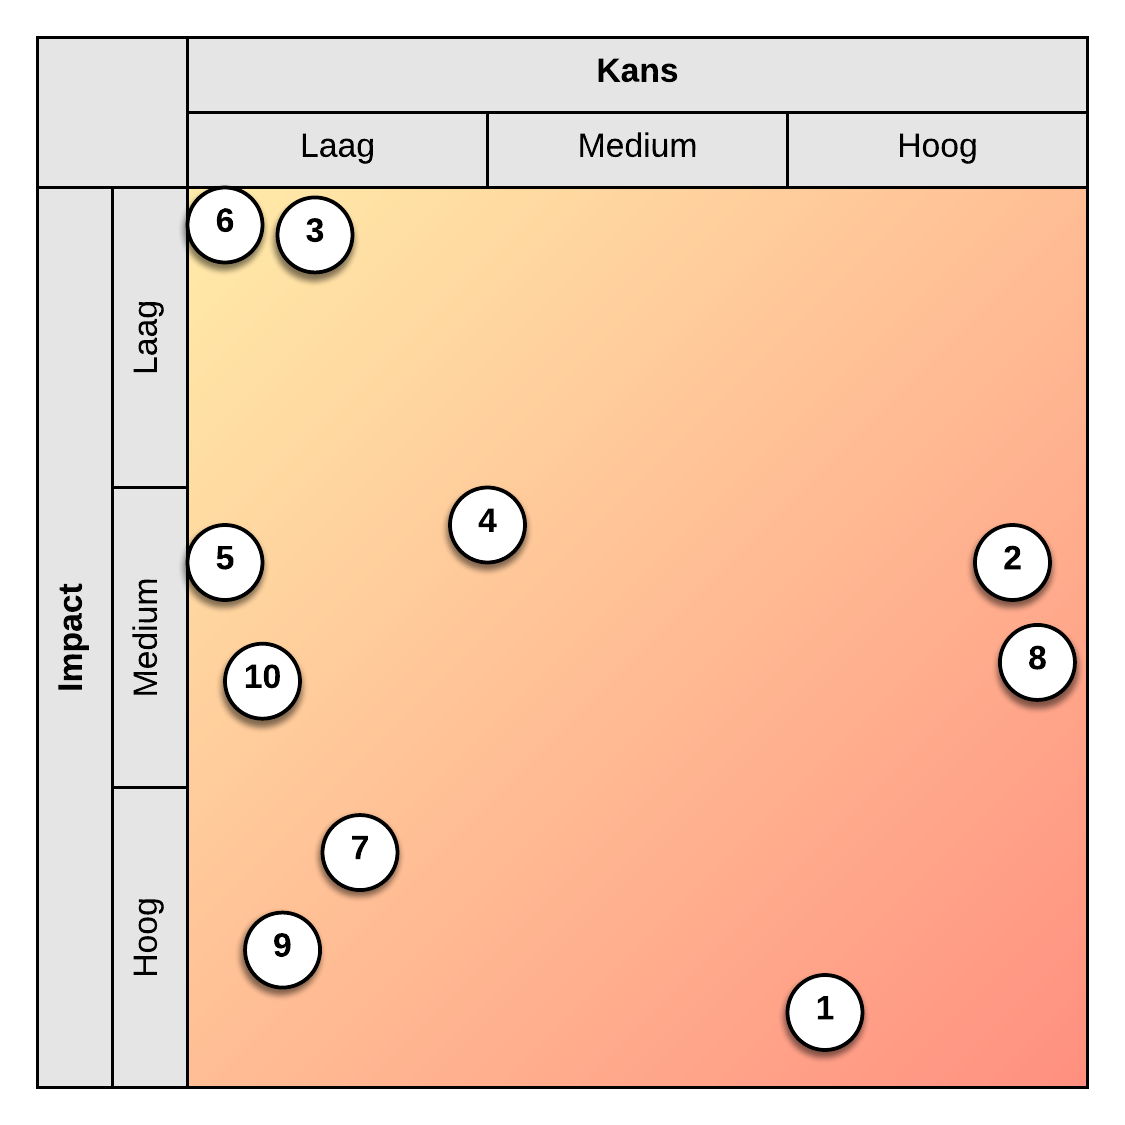
\includegraphics[width=0.75\textwidth]{risicos}
    \caption{Visuale weergave betrouwbaarheidsrisico's SFC}
    \label{fig:risicos}
\end{figure}

\noindent
\textit{Legenda:}
\begin{enumerate}
    \item Verrijking door het onjuist vastleggen van de marge. Bijvoorbeeld door onvolledigheid van de genoten inkoopkortingen, door onjuiste registratie van verkoopkortingen, of door het verantwoorden van perioden met hoge prijzen in perioden met lage prijzen;
    \item Gebrek aan functiescheiding bij het autoriseren van facturen;
    \item Het verval van verkoopcontracten waardoor teveel vreemde valuta is ingedekt;
    \item Bevoegdheid inkopers om impuls te geven en om te beschikken over inkopen;
    \item Samenspanning van inkopers met externe Coldstores;
    \item Ongeoorloofde toegang tot de opslag;
    \item Bevoegdheid tot orderacceptatie en bepaling van kredietwaardigheid afnemer;
    \item Bij afwezigheid worden rechten en gebruikersnamen uitgewisseld om het werk door te kunnen zetten;
    \item Bevoegdheid om assortiment- of prijswijzigingen door te voeren;
    \item Juistheid en volledigheid van klant- en ordergegevens.
\end{enumerate}




